\section*{Simulations}
\label{sec:sim}

Our simulations hypothesize two prey species, and five time points.  Of the hierarchy of hypotheses, we simulate data under three null hypotheses: $\{c_s, c_t\}$.  Sample sizes are chosen randomly from four overlapping levels.  Let ``small'' sample sizes be randomly sampled numbers in $[20,50]$, ``medium'' encompass $[30,75]$, ``large'' $[50,150]$, and ``huge'' $[100,200]$.  Hence, we randomly sample prey and predator gut count observations for each time period from one of the sample size levels, then cycle through all hypotheses.  This is repeated for each level of sample size.  We simulate data for each of the $8$ scenarios above under both the standard maximum likelihood theory and under the EM algorithm.  Only the details of the EM algorithm are presented here, as the other simulations only reinforce the theory of point estimation; that our estimators are uniformly minimum-variance and unbiased (UMVUE).

For all simulated data, the true parameter values for the rate at which prey species are encountered in the wild are fixed to be $\gamma_{st} := \pi, \, \forall s,t$. The values of $\lambda_{st}$ are set for each null hypothesis.  Under the hypothesis $c_s$, the ratio of rates varies by species $s$ only, so we put $\lambda_{1t} := \sqrt{2}$ and $\lambda_{2t} := \pi$.  Hence, $c_1 := \sqrt{2}/\pi \approx 0.45$ and $c_2 := 1$.  For the second hypothesis, the ratio of rates varies by time $t$.  Here, we put $\lambda_{st} := t$ for $t \in \{1, \ldots, 5 \}$.  

As noted above we find that the EM algorithm performs well when the parameter values of $\lambda_{st} = \xi(c_{st})\gamma_{st}$ are small.  Figure~\ref{fig:em} contains density plots of the EM algorithm's estimates for the values $c_s,c_t$ for small and huge sample sizes, respectively.  When data are simulated under the null hypothesis $c_s$, we find, even for the small sample size that point estimates of $c_s$ are quite accurate.  Though, when the values of $\lambda_{st}$ are large enough to make $0$s in the simulated data less common, the algorithm occasionally over-estimates the true values of $c_t$ despite the increased sample size.  The plots of $\gamma_{st}$ under the EM algorithm are not given as we do not consider missing data in the estimation of these parameters, hence they are UMVUE as before. 

\begin{figure}
  \centering
  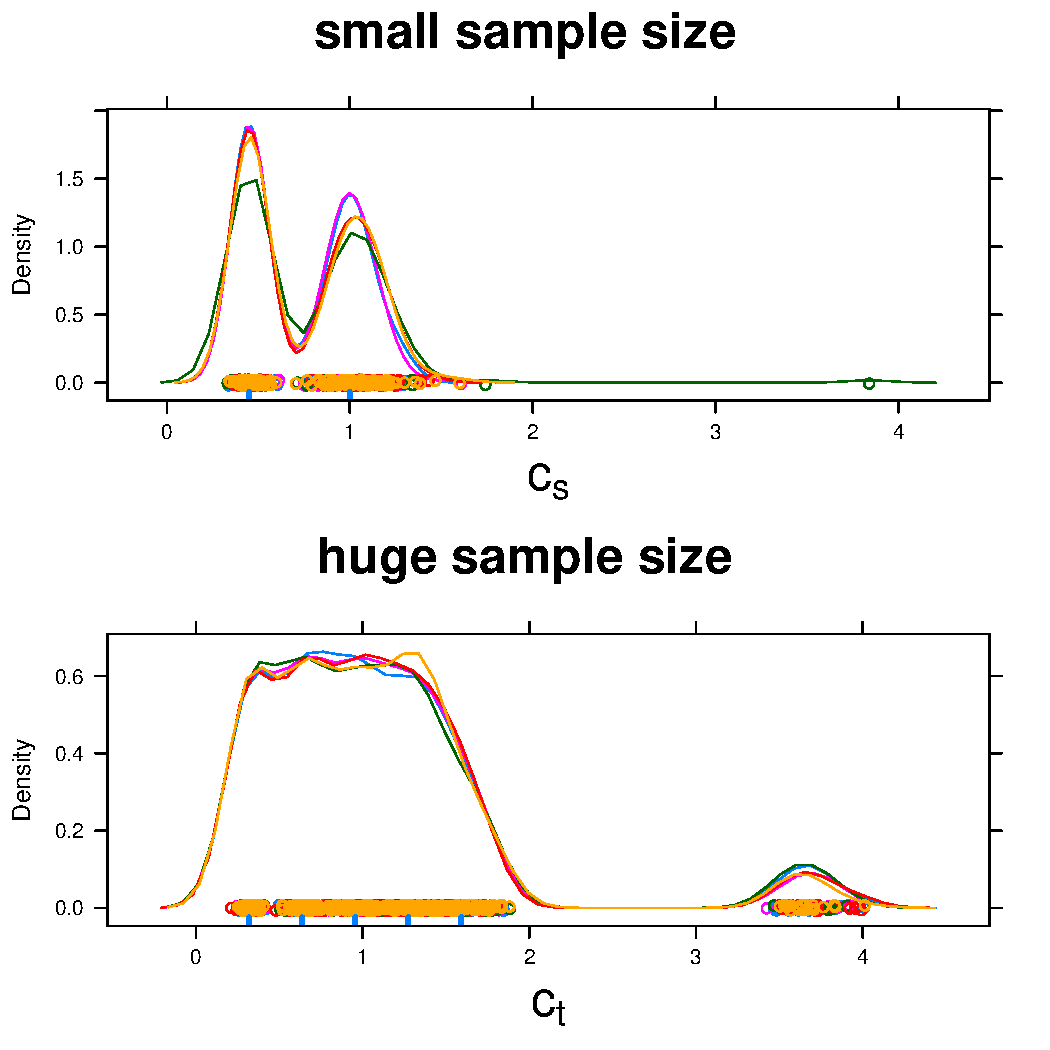
\includegraphics[scale=0.5]{em.pdf}
  \caption{Density plots of the EM algorithm's estimates of $c_s$ and $c_t$ with small and huge sample sizes, respectively.  The estimates near $4$ for both of the plots represent samples for which few zeros appeared in the data and the EM algorithm had a particularly difficult time estimating the true parameter value.}
  \label{fig:em}
\end{figure}










%%% Local Variables: 
%%% mode: latex
%%% TeX-master: "main"
%%% End: 
